\documentclass[a4paper, 12pt]{article}
\usepackage[utf8]{inputenc}
\usepackage[T1]{fontenc}
\usepackage{graphicx}
\usepackage{lipsum}
\usepackage{geometry}
\usepackage{titlesec}
\usepackage{times}
\usepackage{hyperref}
\usepackage{amsmath}
\usepackage[linesnumbered,ruled,vlined]{algorithm2e}
\usepackage{listings}
\usepackage{color}
\usepackage{fancyhdr}
\geometry{a4paper, margin=0.75in}
%\geometry{left=2.5cm, right=2.5cm, top=2.5cm, bottom=2.5cm}
\pagestyle{fancy}
\fancyhf{} % Clear all header and footer fields
\fancyhead[L]{<AppointDoc>}
\fancyhead[C]{Software Requirement Specifications } % Centrally aligned header
\fancyhead[R]{<Version 1.0>}
\fancyfoot[C]{\thepage} % Centrally aligned footer with page number
\definecolor{codegreen}{rgb}{0,0.6,0}
\definecolor{codegray}{rgb}{0.5,0.5,0.5}
\definecolor{codepurple}{rgb}{0.58,0,0.82}
\definecolor{backcolour}{rgb}{0.95,0.95,0.92}

\lstdefinestyle{mystyle}{
    backgroundcolor=\color{backcolour},
    commentstyle=\color{codegreen},
    keywordstyle=\color{magenta},
    numberstyle=\tiny\color{codegray},
    stringstyle=\color{codepurple},
    basicstyle=\ttfamily\footnotesize,
    breakatwhitespace=false,
    breaklines=true,
    captionpos=b,
    keepspaces=true,
    numbers=left,
    numbersep=5pt,
    showspaces=false,
    showstringspaces=false,
    showtabs=false,
    tabsize=2
}

\lstset{style=mystyle}
\begin{document}
\begin{titlepage}
    \centering
    \vspace{3.5cm}
    
\includegraphics[width=0.5\textwidth]{FAST.png}\par\vspace{1cm}
    
\includegraphics[width=0.5\textwidth]{NU-logo.jpg}\par\vspace{1cm}
    \vspace{1.5cm}
    {\scshape\LARGE\textbf {Software Requirement Specifications} \par}
    \vspace{1.5cm}
    {\scshape\LARGE\textbf {AppointDoc\\Doctor Appointment System\\} \par}
    {\scshape\Large Version 1.0 \par}
    \vspace{1.5cm}
    {\scshape\Large Instructor Ms. Javeria Farooq (BCS-6E)\\ \par}
    {\scshape\Large Software Engineering (CS-3009) \par}
    \vspace{1.5cm}
    \begin{itemize}
    \item {\scshape\Large Muhammad Hamza (K21-4579) \par}
    \vspace{0.12cm}
    \item {\scshape\Large Muhammad Salar (K21-4619) \par}
    \vspace{0.12cm}
    \item {\scshape\Large Emmanuel (K21-4871) \par}
    \vspace{0.12cm}
    \item {\scshape\Large Ritesh Kumar (K21-3961) \par}
    \end{itemize}
    \vfill   
    {Foundation of Advancement of Science and Technology \par}
    {National University of Computer and Emerging Sciences \par}
    {Department of Computer Science \par}
    {Karachi, Pakistan \par}
    {Sunday, March 31, 2024 \par}
\end{titlepage}

\tableofcontents
\newpage

\section*{\centering SOFTWARE REQUIREMENT SPECIFICATIONS}

\section{Introduction}

\subsection{Motivation}
The APPOINTDOC system aims to streamline the process of scheduling and managing doctor appointments. In today's fast-paced healthcare environment, efficient appointment management is crucial for both patients and medical practitioners. By providing an intuitive and reliable platform, APPOINTDOC seeks to enhance the patient experience and optimize doctors' schedules.

\subsection{Stakeholders}
The following stakeholders are involved in the APPOINTDOC system:

\begin{itemize}
    \item \textbf{Patients}:
    \begin{itemize}
        \item Users seeking medical appointments.
        \item Primary interaction: Booking, rescheduling, and canceling appointments.
        \item Requirement elicitation: Through user interviews and feedback.
    \end{itemize}
    
    \item \textbf{Doctors and Medical Staff}:
    \begin{itemize}
        \item Responsible for managing appointments.
        \item Primary interaction: Viewing schedules, confirming appointments.
        \item Requirement elicitation: Interviews with doctors and staff.
    \end{itemize}
    
    \item \textbf{Administrators}:
    \begin{itemize}
        \item Oversee system configuration, user management, and security.
        \item Primary interaction: Managing user accounts, system settings.
        \item Requirement elicitation: Interviews with hospital administrators.
    \end{itemize}
    
    \item \textbf{Developers}:
    \begin{itemize}
        \item Technical team responsible for system design, development, and maintenance.
        \item Primary interaction: Implementing features, ensuring system functionality.
        \item Requirement elicitation: Collaboration with other stakeholders.
    \end{itemize}
\end{itemize}

\subsection{Assumptions and Dependencies}
To ensure successful implementation, we make the following assumptions and dependencies:

\begin{itemize}
    \item \textbf{Reliable Internet Connectivity}: Users have access to stable internet connections for seamless interaction with the system.
    \item \textbf{Integration with Existing Systems}: APPOINTDOC integrates with hospital databases for patient records and other relevant data.
    \item \textbf{Compliance with Healthcare Regulations}: The system adheres to privacy laws and other healthcare-related regulations.
\end{itemize}

\section{Functional Requirements}

\subsection{Appointment Booking}
\subsubsection{Feature: Book Appointment}
\begin{itemize}
    \item \textbf{Description}: Patients can schedule appointments with specific doctors on preferred dates and times.
    \item \textbf{User Interaction}: Patients provide their details, select a doctor, and choose an available time slot.
    \item \textbf{System Behavior}: The system confirms the appointment and updates the doctor's schedule.
\end{itemize}

\subsubsection{Feature: View Appointments}
\begin{itemize}
    \item \textbf{Description}: Doctors and staff can view their upcoming appointments.
    \item \textbf{User Interaction}: Doctors log in and access their appointment list.
    \item \textbf{System Behavior}: Displays a list of scheduled appointments with patient details.
\end{itemize}

\subsection{Appointment Management}
\subsubsection{Feature: Cancel Appointment}
\begin{itemize}
    \item \textbf{Description}: Patients can cancel booked appointments.
    \item \textbf{User Interaction}: Patients log in, select the appointment, and cancel.
    \item \textbf{System Behavior}: Updates the appointment status and notifies the doctor.
\end{itemize}

\subsubsection{Feature: Reschedule Appointment}
\begin{itemize}
    \item \textbf{Description}: Patients can request to reschedule appointments.
    \item \textbf{User Interaction}: Patients provide reasons and preferred new time slots.
    \item \textbf{System Behavior}: Notifies the doctor and suggests alternative slots.
\end{itemize}

\section{Non-Functional Requirements}

\subsection{Performance}
\begin{itemize}
    \item \textbf{Response Times}: The system should respond within seconds for most interactions.
    \item \textbf{Throughput}: Handle concurrent users during peak hours.
\end{itemize}

\subsection{Reliability}
\begin{itemize}
    \item \textbf{Availability}: The system should be available 24/7, with minimal downtime for maintenance.
    \item \textbf{Fault Tolerance}: Regularly back up appointment data to prevent loss.
\end{itemize}

\subsection{Security}
\begin{itemize}
    \item \textbf{Authentication}: Users must log in with valid credentials.
    \item \textbf{Authorization}: Role-based access control (patient, doctor, admin).
    \item \textbf{Data Privacy}: Protect patient information according to privacy laws.
\end{itemize}

\subsection{Usability}
\begin{itemize}
    \item \textbf{Accessibility}: Ensure the system is usable by people with different needs.
    \item \textbf{User Interface Design}: Intuitive and consistent design for easy navigation.
\end{itemize}

\subsection{Other}
\begin{itemize}
    \item \textbf{Scalability}: Design the system to accommodate future growth.
    \item \textbf{Data Privacy}: Protect patient information (compliance with privacy laws).
    \item \textbf{Auditability}: Maintain detailed logs for troubleshooting and accountability.
    \item \textbf{Error Handling}: Clear procedures for unexpected scenarios.
\end{itemize}

\section{Constraints}
\subsection{Budget Constraints}
\begin{itemize}
    \item The project must operate within a specified budget.
    \item Optimize costs while delivering essential features.
\end{itemize}

\subsection{Time Constraints}
\begin{itemize}
    \item Develop and deploy the system within the agreed timeframe.
    \item Use agile methodologies to manage time effectively.
\end{itemize}

\subsection{Resource Constraints}
\begin{itemize}
    \item Personnel availability (developers, designers).
    \item Infrastructure capacity (servers, network).
    \item Software tools (licensing, open-source alternatives).
\end{itemize}

\subsection{Risk Constraints}
\begin{itemize}
    \item Identify and manage project risks proactively.
\end{itemize}

\subsection{Technology Constraints}
\begin{itemize}
    \item Compatibility with existing systems.
    \item Choose technologies with long-term support.
\end{itemize}

\subsection{Compliance Constraints}
\begin{itemize}
    \item Legal and regulatory compliance (data privacy, healthcare laws).
\end{itemize}

\subsection{Organizational Structure Constraints}
\begin{itemize}
    \item Clear communication channels and decision-making processes.
\end{itemize}

\section{Architecture Design Overview}
The APPOINTDOC system architecture includes several high-level components that interact seamlessly to create a robust and efficient doctor appointment system:

\subsection{User Interface (UI)}
\begin{itemize}
    \item The \textbf{UI} serves as the primary interaction point for users (patients, doctors, and administrators).
    \item Key features include:
    \begin{itemize}
        \item \textbf{Appointment Booking}: Patients can easily schedule appointments by selecting doctors, preferred dates, and available time slots.
        \item \textbf{View Appointments}: Doctors and staff access their upcoming appointment lists, including patient details.
        \item \textbf{Cancellation and Rescheduling}: Patients can cancel or request rescheduling of appointments.
    \end{itemize}
\end{itemize}

\subsection{Backend Services}
\begin{itemize}
    \item The \textbf{Backend Services} layer handles critical business logic and system functionality.
    \item Responsibilities:
    \begin{itemize}
        \item \textbf{Authentication and Authorization}: Validates user credentials and controls access based on roles (patient, doctor, admin).
        \item \textbf{Appointment Management}: Manages appointment scheduling, availability, and notifications.
        \item \textbf{Data Processing}: Processes user requests, updates schedules, and communicates with the database.
    \end{itemize}
\end{itemize}

\subsection{Database}
\begin{itemize}
    \item The \textbf{Database} stores essential data related to appointments, patients, doctors, and administrative settings.
    \item Components:
    \begin{itemize}
        \item \textbf{Appointment Records}: Store details of scheduled appointments (patient ID, doctor ID, date, time).
        \item \textbf{User Profiles}: Maintain user information (name, contact details, role).
        \item \textbf{Doctor Schedules}: Track doctors' availability.
    \end{itemize}
\end{itemize}

\subsection{Authentication and Authorization}
\begin{itemize}
    \item \textbf{Authentication} ensures secure access to the system:
    \begin{itemize}
        \item Users log in with valid credentials (username/password or other authentication methods).
        \item Sessions are managed securely.
    \end{itemize}
    \item \textbf{Authorization} controls user permissions:
    \begin{itemize}
        \item Role-based access (patient, doctor, admin).
        \item Fine-grained permissions for specific features (e.g., only doctors can view patient medical history).
    \end{itemize}
\end{itemize}

\subsection{Notification Service}
\begin{itemize}
    \item The \textbf{Notification Service} keeps users informed:
    \begin{itemize}
        \item \textbf{Appointment Reminders}: Sends reminders to patients and doctors before scheduled appointments.
        \item \textbf{Critical Alerts}: Notifies administrators about system events (e.g., server downtime, security breaches).
    \end{itemize}
\end{itemize}

\subsection{Integration with Existing Systems}
\begin{itemize}
    \item APPOINTDOC integrates seamlessly with other hospital systems:
    \begin{itemize}
        \item \textbf{Patient Records}: Integrates with existing databases to retrieve patient information.
        \item \textbf{Billing and Insurance}: Shares relevant data for billing and insurance purposes.
        \item \textbf{Electronic Health Records (EHR)}: Ensures consistency across systems.
    \end{itemize}
\end{itemize}


\subsection{Component Diagram}

\subsubsection{MERN Stack}
\begin{center}
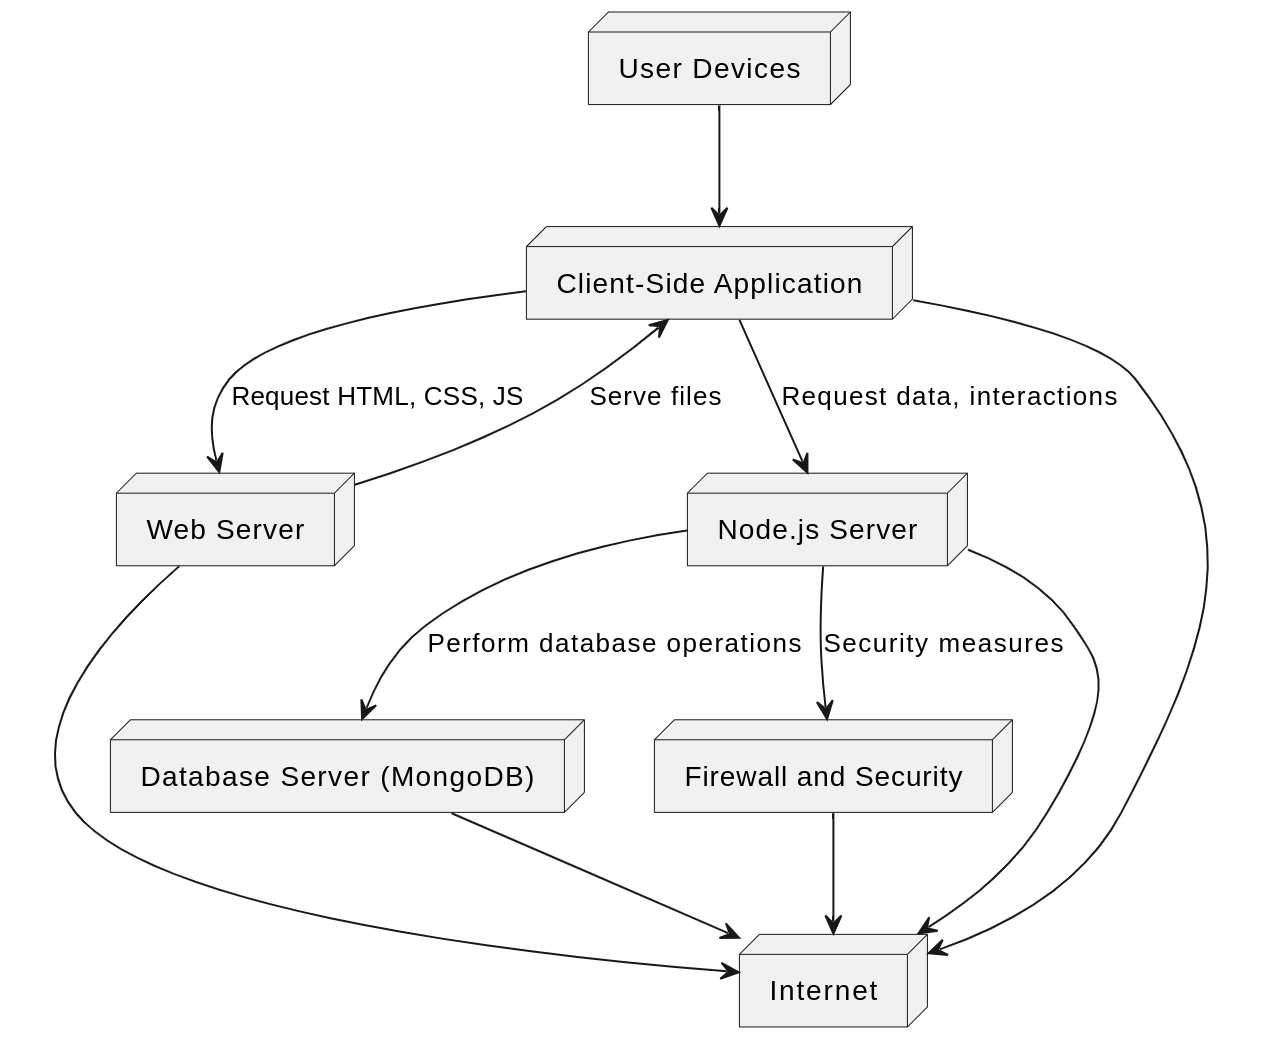
\includegraphics[width=1\textwidth]{component.png}\par
\end{center}
\begin{itemize}
    \item \textbf{User Devices}:
    \begin{itemize}
        \item Represents devices (such as laptops, smartphones, tablets) used by end-users (patients, doctors, administrators).
        \item Interacts with the client-side application.
    \end{itemize}
    
    \item \textbf{Client-Side Application (React)}:
    \begin{itemize}
        \item The front-end part of the MERN stack.
        \item Responsible for rendering UI components, handling user interactions, and making requests to the server.
        \item Communicates with the Node.js server via RESTful APIs.
    \end{itemize}
    
    \item \textbf{Web Server (Node.js)}:
    \begin{itemize}
        \item Serves the client-side application to user devices.
        \item Handles incoming HTTP requests from clients.
        \item Routes requests to appropriate endpoints (API routes).
    \end{itemize}
    
    \item \textbf{Node.js Server (Express)}:
    \begin{itemize}
        \item The back-end part of the MERN stack.
        \item Manages business logic, data processing, and database interactions.
        \item Implements RESTful APIs for CRUD operations (Create, Read, Update, Delete).
    \end{itemize}
    
    \item \textbf{Database Server (MongoDB)}:
    \begin{itemize}
        \item Stores data related to appointments, user profiles, and other system information.
        \item MongoDB is a NoSQL database used for its flexibility and scalability.
        \item Communicates with the Node.js server to retrieve or update data.
    \end{itemize}
    
    \item \textbf{Firewall and Security}:
    \begin{itemize}
        \item Ensures network security by controlling incoming and outgoing traffic.
        \item Protects against unauthorized access and potential threats.
        \item May include security measures like authentication, authorization, and encryption.
    \end{itemize}
    
    \item \textbf{Internet}:
    \begin{itemize}
        \item Represents the global network infrastructure.
        \item Facilitates communication between user devices, web servers, and database servers.
    \end{itemize}
\end{itemize}

\newpage
\subsubsection{Doctor Appointment System}
\begin{center}
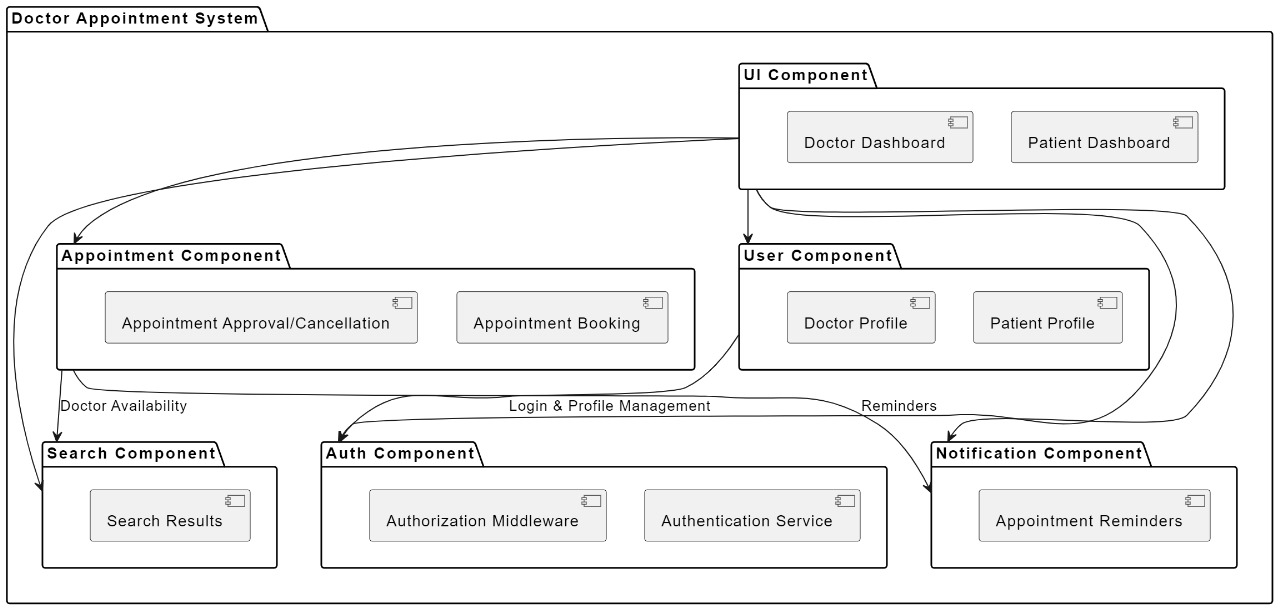
\includegraphics[width=1\textwidth]{component.jpeg}\par
\end{center}
\begin{itemize}
    \item \textbf{UI (User Interface)}
    \begin{itemize}
        \item Represents the visual part of the system that users interact with.
        \item Responsible for displaying appointment-related information to patients and doctors.
        \item Includes features like appointment booking forms, appointment lists, and notifications.
    \end{itemize}
    
    \item \textbf{User}
    \begin{itemize}
        \item Represents the end-users of the system (patients, doctors, and administrators).
        \item Interacts with the UI to perform actions such as booking appointments, viewing schedules, and managing appointments.
    \end{itemize}
    
    \item \textbf{Appointment Component}
    \begin{itemize}
        \item Manages all aspects related to appointments:
        \begin{itemize}
            \item Booking: Allows patients to schedule appointments.
            \item Cancellation: Allows patients to cancel appointments.
            \item Rescheduling: Handles requests from patients to change appointment times.
            \item Communicates with the database to update appointment records.
        \end{itemize}
    \end{itemize}
    
    \item \textbf{Search Component}
    \begin{itemize}
        \item Responsible for searching and retrieving relevant information:
        \begin{itemize}
            \item Patient search: Allows doctors and administrators to find patient records.
            \item Doctor availability search: Helps patients find available time slots for specific doctors.
        \end{itemize}
    \end{itemize}
    
    \item \textbf{Auth (Authentication) Component}
    \begin{itemize}
        \item Ensures secure access to the system:
        \begin{itemize}
            \item Validates user credentials during login.
            \item Manages user sessions.
            \item Role-based access control: Differentiates between patients, doctors, and administrators.
        \end{itemize}
    \end{itemize}
    
    \item \textbf{Notification Component}
    \begin{itemize}
        \item Sends notifications to users:
        \begin{itemize}
            \item Appointment reminders: Alerts patients and doctors before scheduled appointments.
            \item Critical alerts: Notifies administrators about system events (e.g., server issues).
        \end{itemize}
    \end{itemize}
    
    \item \textbf{Integration with Existing Systems}
    \begin{itemize}
        \item Connects with other hospital systems:
        \begin{itemize}
            \item Patient records: Retrieves patient information from existing databases.
            \item Billing and insurance systems: Shares relevant data for billing purposes.
            \item Electronic Health Records (EHR): Ensures consistency across systems.
        \end{itemize}
    \end{itemize}
\end{itemize}

\newpage
\subsection{Deployment Diagram}
\begin{center}
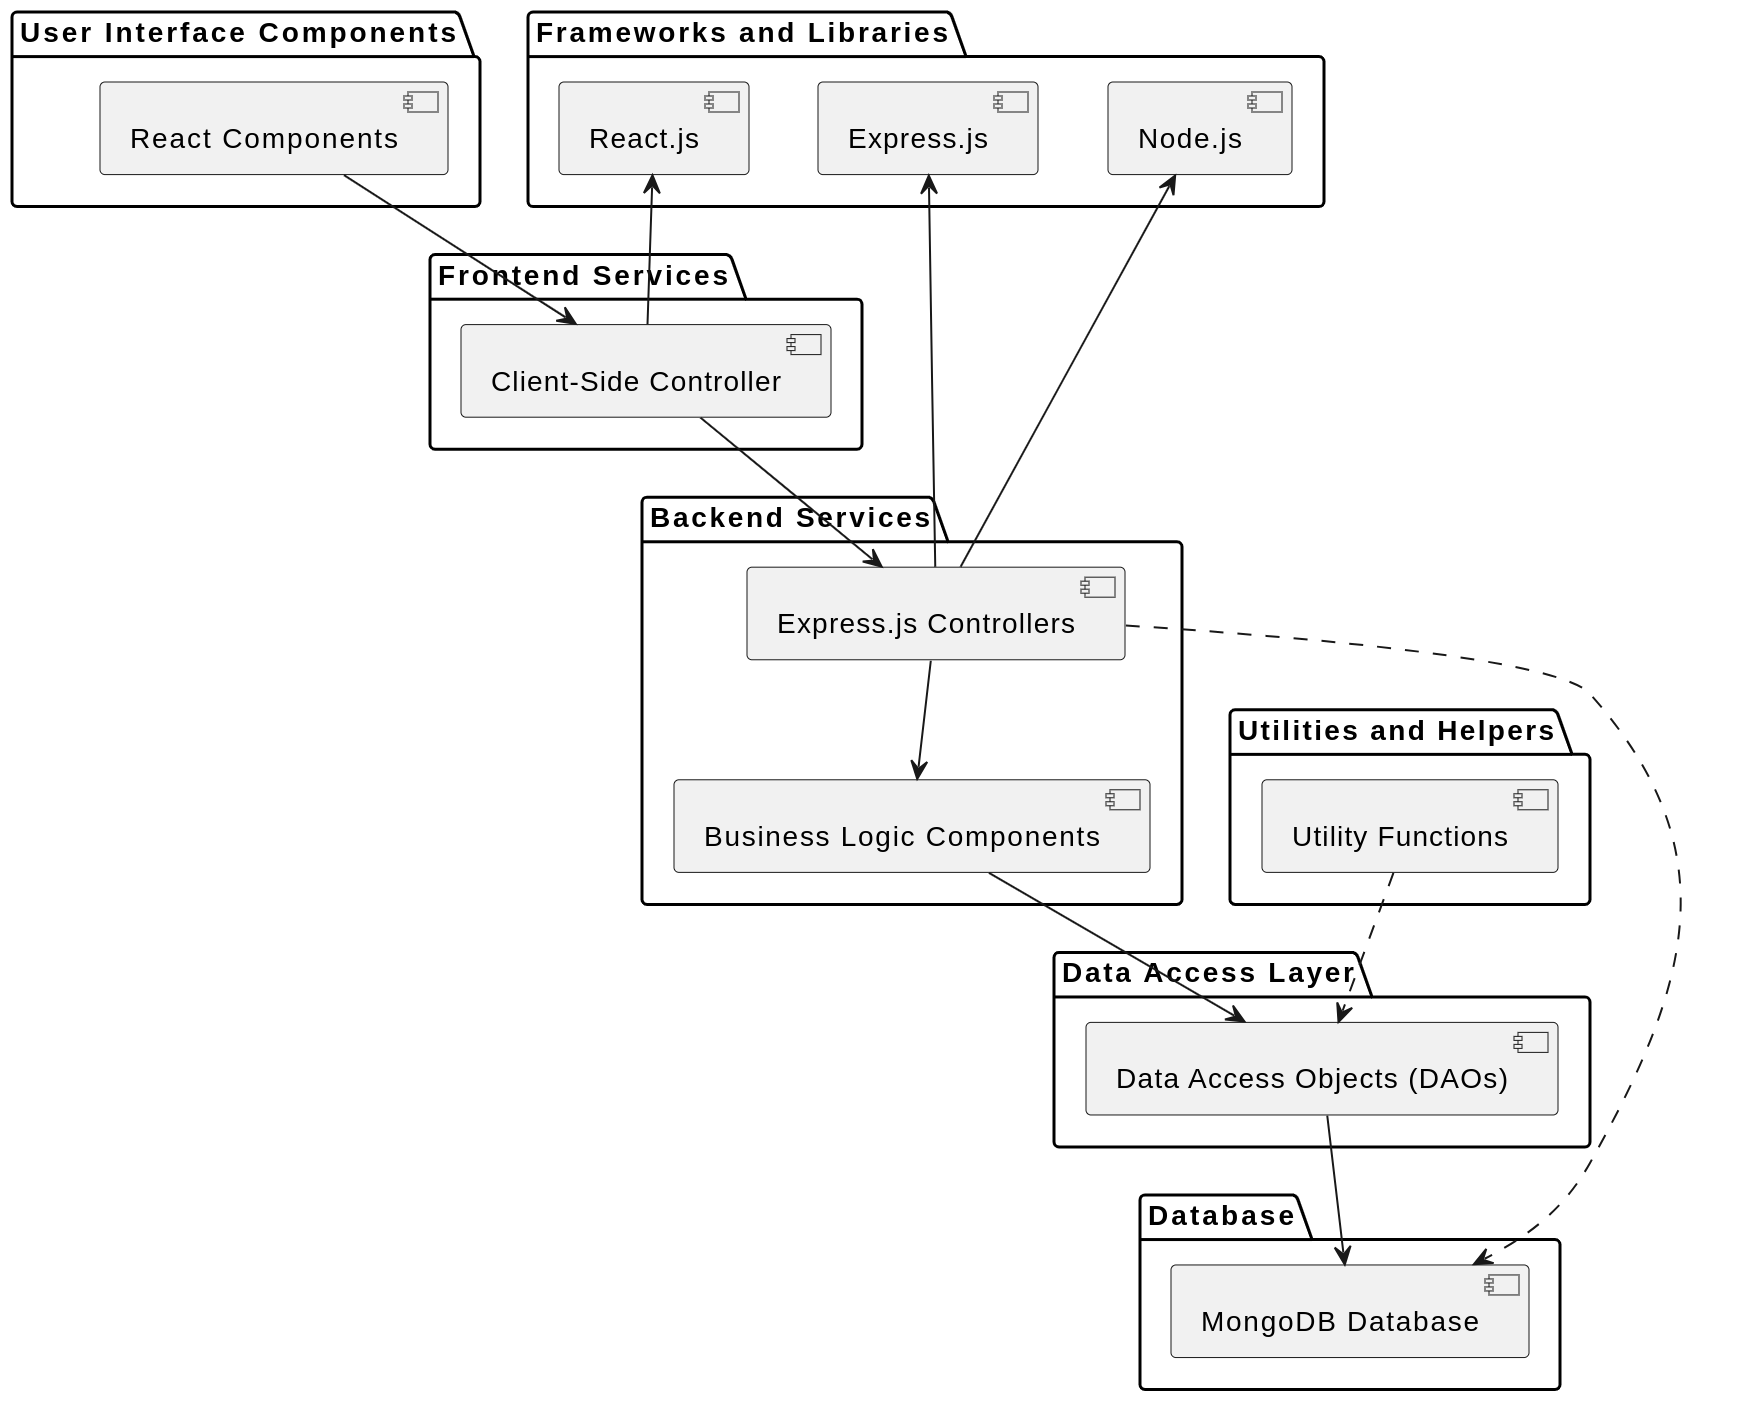
\includegraphics[width=1\textwidth]{deployment.png}\par
\end{center}
\begin{itemize}
    \item \textbf{User Devices}:
    \begin{itemize}
        \item Represents devices (such as laptops, smartphones, tablets) used by end-users (patients, doctors, administrators).
        \item Interacts with the client-side application.
    \end{itemize}
    
    \item \textbf{Client-Side Application (React)}:
    \begin{itemize}
        \item The front-end part of the MERN stack.
        \item Responsible for rendering UI components, handling user interactions, and making requests to the server.
        \item Communicates with the Node.js server via RESTful APIs.
    \end{itemize}
    
    \item \textbf{Web Server (Node.js)}:
    \begin{itemize}
        \item Serves the client-side application to user devices.
        \item Handles incoming HTTP requests from clients.
        \item Routes requests to appropriate endpoints (API routes).
    \end{itemize}
    
    \item \textbf{Node.js Server (Express)}:
    \begin{itemize}
        \item The back-end part of the MERN stack.
        \item Manages business logic, data processing, and database interactions.
        \item Implements RESTful APIs for CRUD operations (Create, Read, Update, Delete).
    \end{itemize}
    
    \item \textbf{Database Server (MongoDB)}:
    \begin{itemize}
        \item Stores data related to appointments, user profiles, and other system information.
        \item MongoDB is a NoSQL database used for its flexibility and scalability.
        \item Communicates with the Node.js server to retrieve or update data.
    \end{itemize}
    
    \item \textbf{Firewall and Security}:
    \begin{itemize}
        \item Ensures network security by controlling incoming and outgoing traffic.
        \item Protects against unauthorized access and potential threats.
        \item May include security measures like authentication, authorization, and encryption.
    \end{itemize}
    
    \item \textbf{Internet}:
    \begin{itemize}
        \item Represents the global network infrastructure.
        \item Facilitates communication between user devices, web servers, and database servers.
    \end{itemize}
\end{itemize}


\section{Revision History}
\begin{itemize}
    \item Project Proposal Submission (February 21, 2024):
    \begin{itemize}
        \item Submitted the initial project proposal.
        \item Outlined the project’s objectives, scope, and stakeholders.
    \end{itemize}
    
    \item SRS and Prototype Submission (March 31, 2024):
    \begin{itemize}
        \item Submitted the Software Requirements Specification (SRS) document.
        \item Included detailed functional and non-functional requirements.
        \item Provided a prototype and UI design for the system.
    \end{itemize}
\end{itemize}


\newpage
\section*{\centering PROTOTYPE}

\section{User Interface}

\subsection{Doctor Application}
\begin{center}
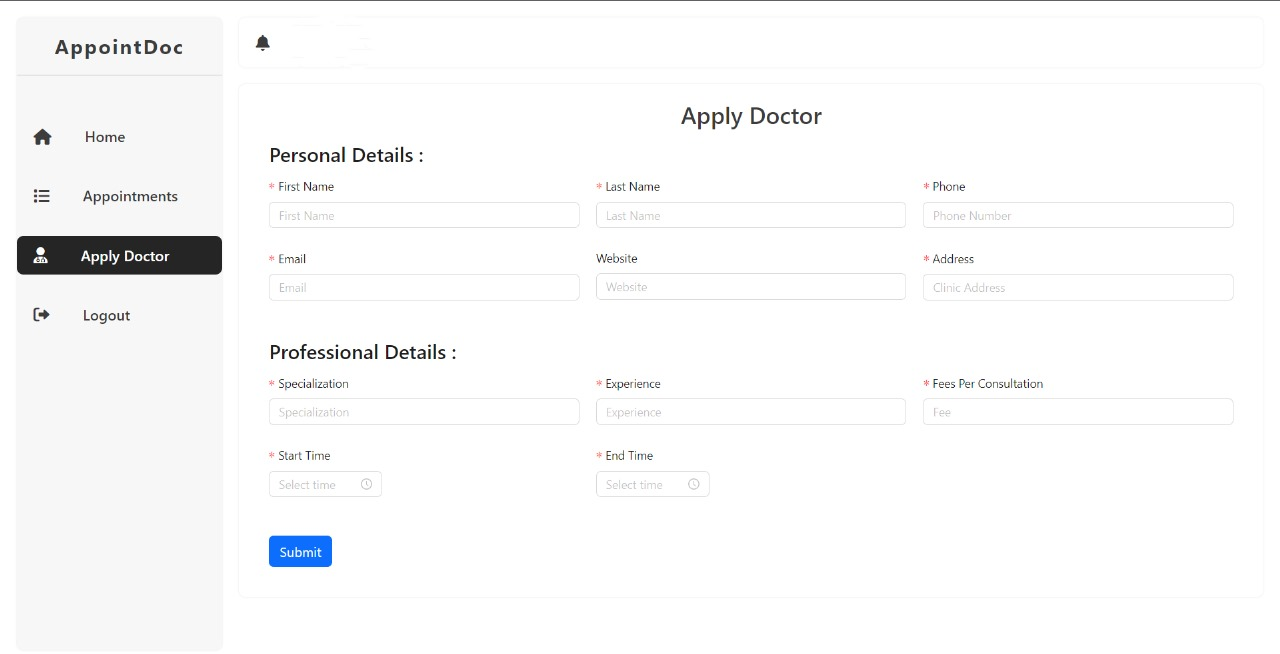
\includegraphics[width=1\textwidth]{apply.jpg}\par
\end{center}

\subsection{Appointments Listing}
\begin{center}
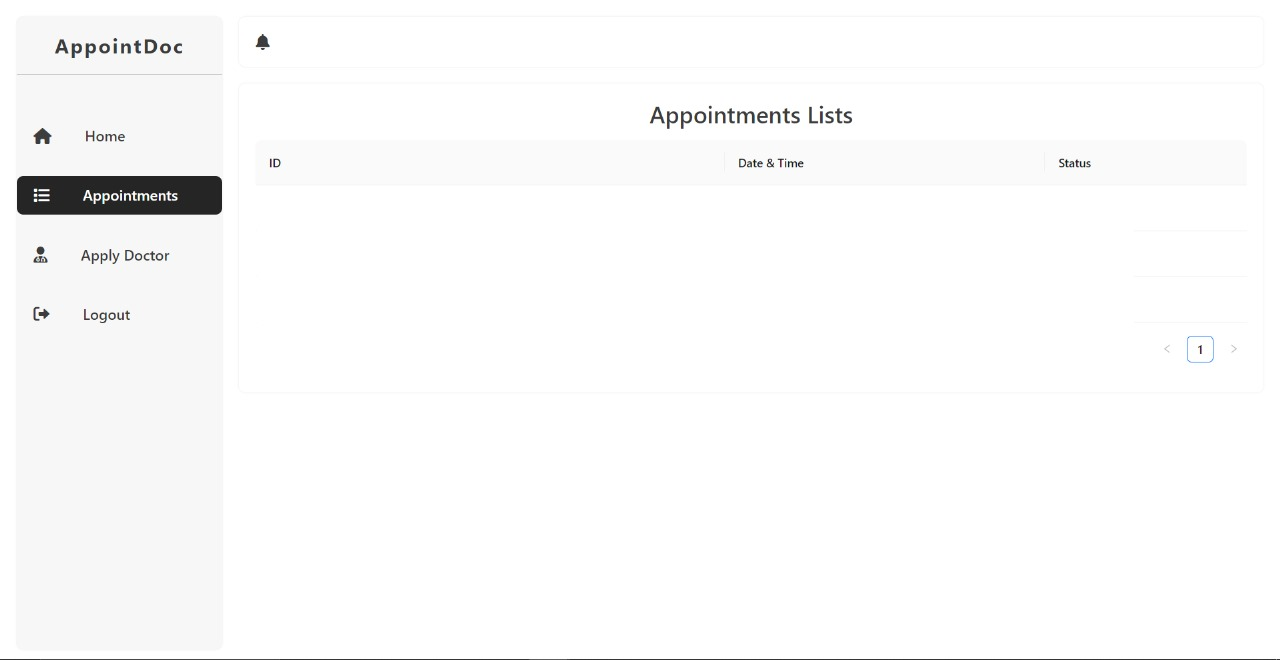
\includegraphics[width=1\textwidth]{appoint.jpg}\par
\end{center}

\subsection{Home Page}
\begin{center}
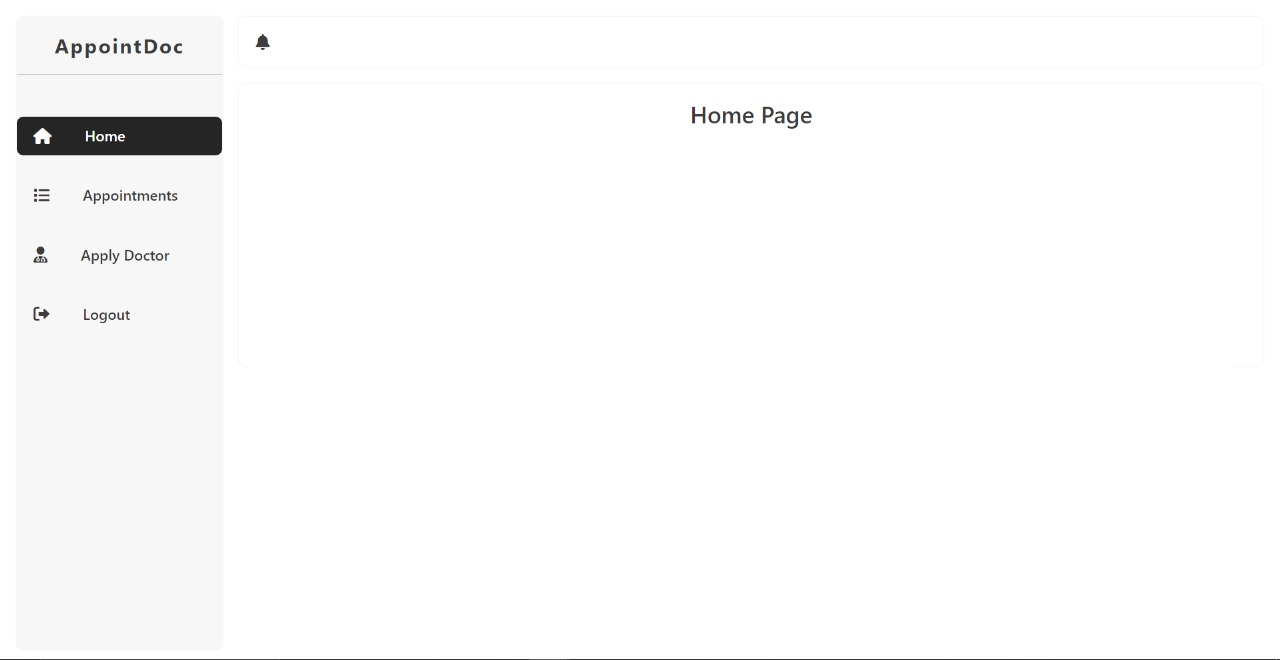
\includegraphics[width=1\textwidth]{home.jpg}\par
\end{center}

\subsection{Appointments Booking}
\begin{center}
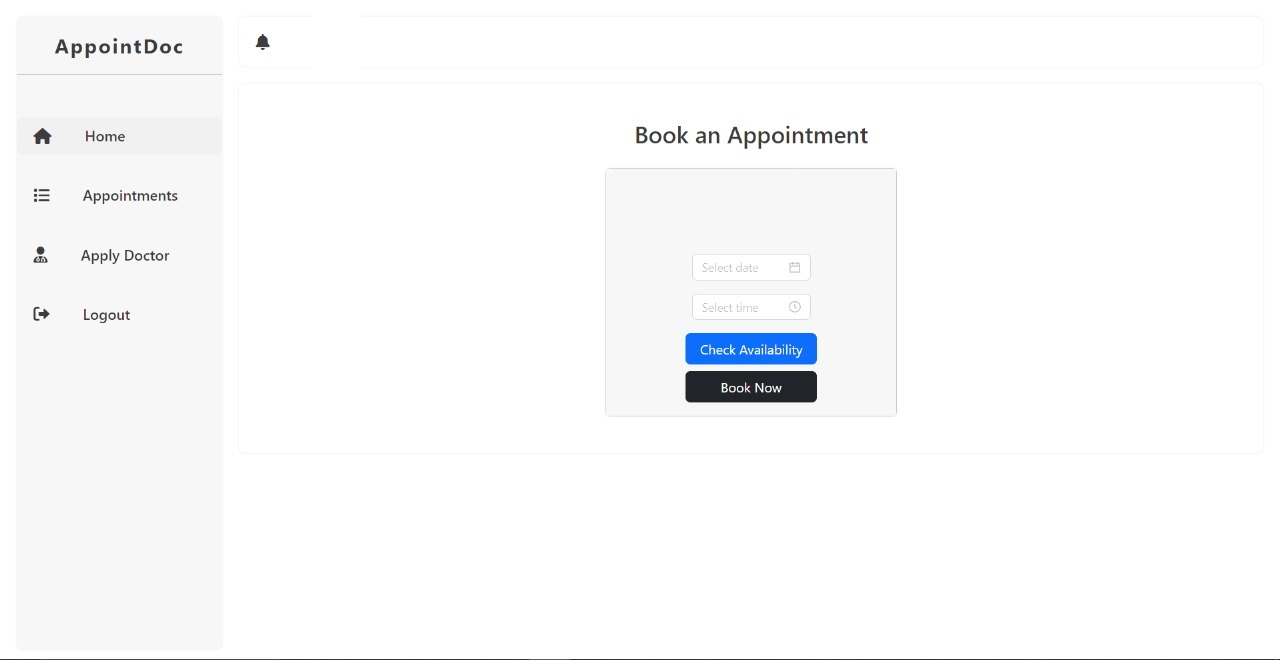
\includegraphics[width=1\textwidth]{login.jpg}\par
\end{center}

\subsection{Notifications Panel}
\begin{center}
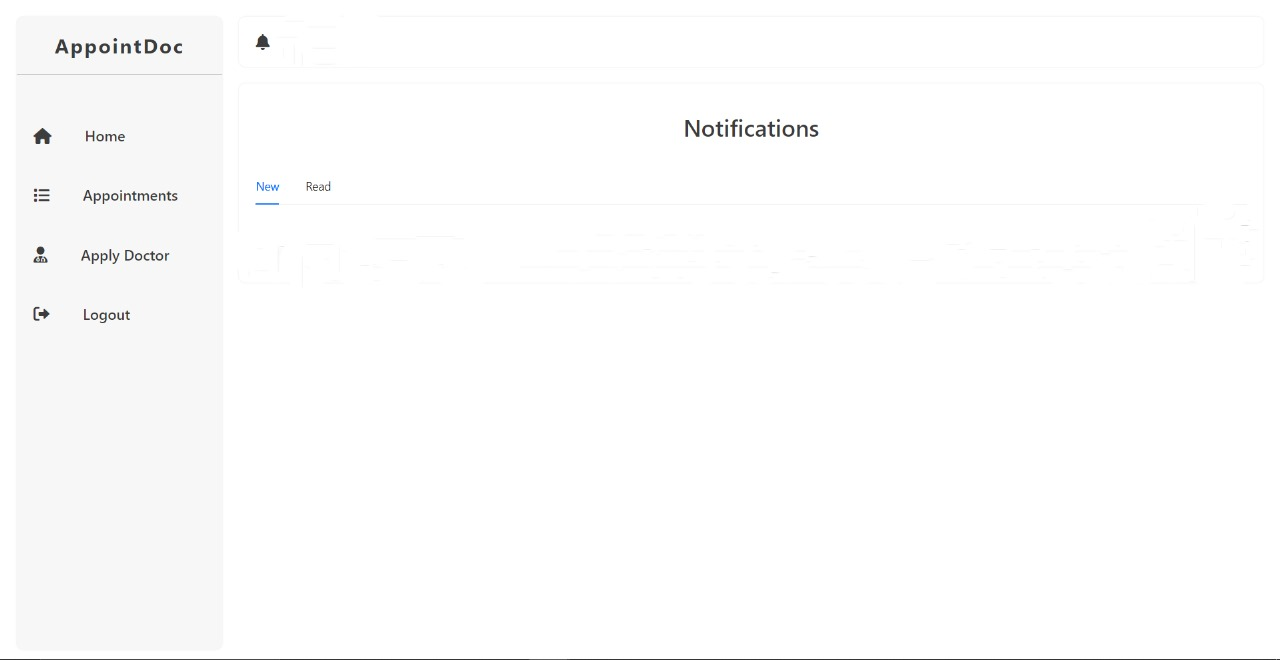
\includegraphics[width=1\textwidth]{noti.jpg}\par
\end{center}

\end{document}